\documentclass[a4paper,12pt]{article}

\usepackage{url}
\usepackage{caption}
\usepackage{subcaption}
\usepackage{graphicx}
\usepackage{wrapfig}
\usepackage{xcolor}
\usepackage{listings}
\begin{document}

\begin{center}
\begin{Large}


\textbf{Assignment 5}

Web Science CS595

Name: Amara Naas
\end{Large}
\end{center}
\pagebreak

\textbf{Answer to question 1}

$\:$

\par
The Python program (q1.py)\footnote{File uploaded to github} will read the file mln.graphml \footnotemark[1] and parse it by using BeautifulSoup and XML element tree. the program will extract only the friend count data for each friend and save it in a file called resultdata.txt\footnotemark[1]. By using the data in the resultdata file I created a graph of the number of friends (y-axis) and the friends sorted by number of friends (x-axis) as shown in figure 1. We can see from figure 1 that friendship paradox holds for mln Facebook account where total number of his friends was 154 with friend count data represented (The friends who do not have friend count are eliminated by using if statement in q1.py program). Also from the resultdata file I computed the mean, standard deviation, and median of the number of friends that mls' friends have as following:
\begin{lstlisting}
	mean = 357.66
	standard deviation = 370.74
	median = 259
\end{lstlisting}
	
\par

\begin{figure}
	\center
		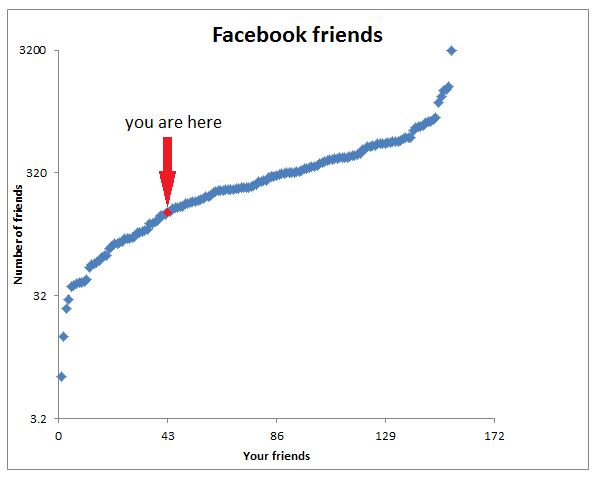
\includegraphics[width=\linewidth]{FaceFriends.png} 
	\caption{Friends count}
\end{figure}

$\:$


\textbf{Answer to question 2}

$\:$

\par
The Python program (q2.py)\footnotemark[1] is a modified program from assignment 1. The only change is in the url value. The program will read all the followers of phonedude\_mln twitter account by extracting only the followers count data for each follower and save it in a file called resultdata1.txt\footnotemark[1]. By using the data in the resultdata1 file I created a graph of the number of followers (y-axis) and the followers sorted by number of followers (x-axis) as shown in figure 2. We can see from figure 2 that friendship paradox holds for phonedude\_mln twitter account where total number of his followers was 196. Also from the resultdata1 file I computed the mean, standard deviation, and median of the number of followers that phonedude\_mln's followers have as following:

\begin{lstlisting}
	mean = 524.3
	standard deviation = 1281
	median = 207
\end{lstlisting}

\par

\begin{figure}
	\center
		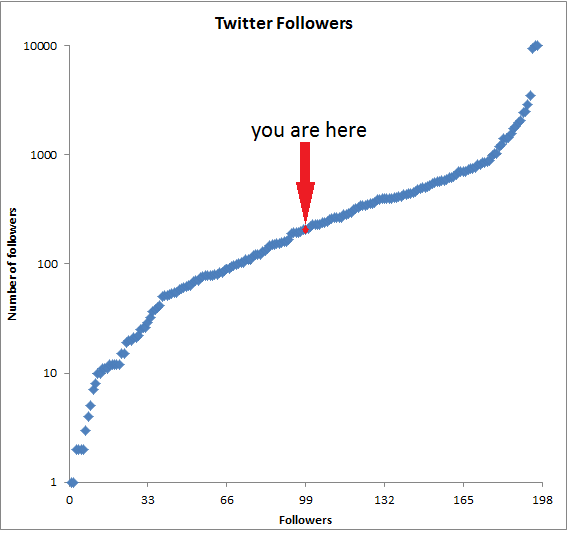
\includegraphics[width=\linewidth]{TwittersFollowers.png} 
	\caption{Followers count}
\end{figure}

%\textcolor{red}{[text]}



\pagebreak

\textbf{Answer to question 3}\par
$\:$

\par
In the Python program (q3.py)\footnote{File uploaded to github} will access linkedIn API and retrieve the data. First thing to do is to create an application, and generate your own access token. Secondly, register the new application, get the consumer key and consumer secret, and save them at the q3.py\footnotemark[2]. Because I do not have friends in linkedIn I only get the my data by generating the Oauth\_Tokens and run q3 python file, and set Oauth\_Token and Oauth\_Token\_Secret as shown in figure 3.
\par

\begin{figure}
	\center
		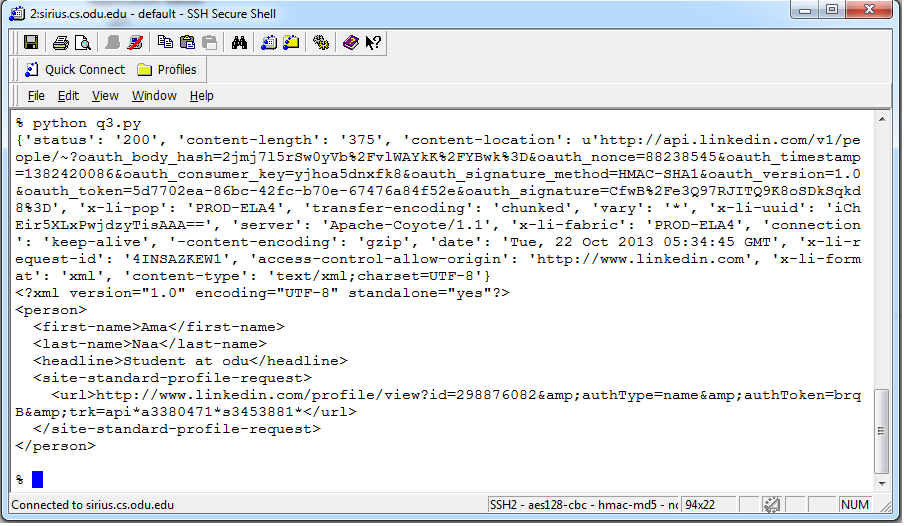
\includegraphics[width=\linewidth]{MyLinkedIn.png} 
	\caption{Followers count}
\end{figure}

$\:$

\textbf{Answer to question 4}\par
$\:$

\par
The Python program (q2.py)\footnotemark[2] is a modified python program from question 2. The only change is in the url value where followers/list is replaced by friends/list. The program will reads all the followings of phonedude\_mln twitter account by extracting only the friends count data for each following and save it in a file called resultdata2.txt\footnotemark[2]. By using the data in the resultdata2 file I created a graph of the number of followings (y-axis) and the followings sorted by number of followings (x-axis) as shown in figure 4. We can see from figure 3 that friendship paradox holds for phonedude\_mln twitter account where total number of his followings was 73. Also from the resultdata2 file I computed the mean, standard deviation, and median of the number of followers that phonedude\_mln's followings have as following:

\begin{lstlisting}
	mean = 323.52
	standard deviation = 455.76
	median = 202
\end{lstlisting}

\par

\begin{figure}
	\center
		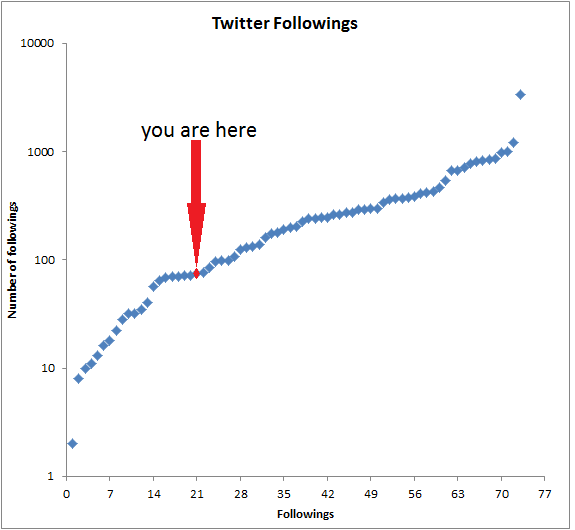
\includegraphics[width=\linewidth]{TwittersFollowings.png} 
	\caption{Followers count}
\end{figure}




\end{document}